\section{SciSpot Design}
\label{sec:design}

%\noindent \textbf{Design Goals:} 
\sysname handles all the cloud resource management and job scheduling associated with running a bag of jobs on transient cloud servers. 
In this section, we look at \sysname's policies for selecting the ``right'' cloud server for a given application, and policies for scheduling and running a bag of jobs on transient servers.
Throughout, our aim is to minimize the overall cost and minimize the impact of preemptions.  \vj{\it have we defined what ``right'' is?, could be useful to define it again here}


\begin{figure}[h]
  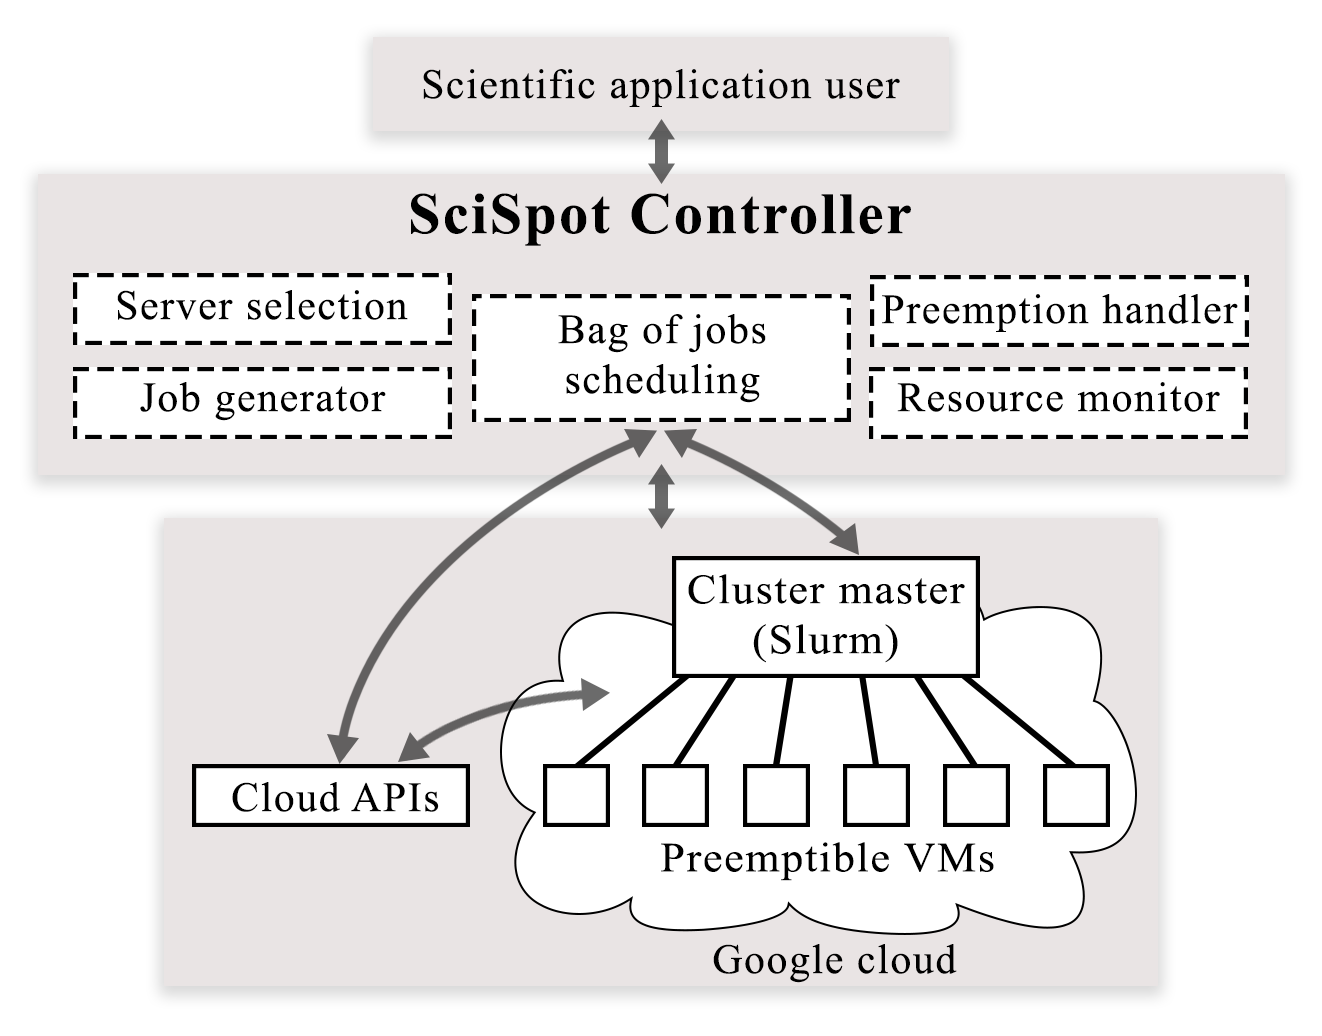
\includegraphics[width=0.3\textwidth]{../figures/Architecture.png}
  \caption{SciSpot Architecture}
  \label{fig:arch}
\end{figure}

\sysname aims to provide a simple user interface to allow users to deploy their applications with minimum changes to their workflow.
Most scientific computing applications are deployed on HPC clusters that have a cluster manager such as Slurm~\cite{slurm} or Torque~\cite{torque}, and \sysname integrates with the cluster manager (e.g., Slurm) to provide the same interface to applications.
As shown in Figure~\ref{fig:arch}, \sysname creates and manages clusters of transient cloud servers, manages all aspects of the VM lifecycle and costs, and implements the various policies described in the rest of this section. 


\noindent \textbf{High-level workflow:} When a user wishes to run a bag of jobs, \sysname handles the provisioning of a cluster of transient cloud servers. In addition, \sysname deals with the scheduling and monitoring of the bag of jobs, and with preemptions.
Execution of a bag of jobs proceeds in two phases. In the first phase, \sysname selects the ``right'' cluster configuration for a given application through a cost-minimizing exploration-based search policy, described in Section~\ref{subsec:server-selection}.
In the second phase, \sysname proceeds to run the remaining jobs in the bag on the optimal cluster configuration. 

\subsection{Server Selection}
\label{subsec:server-selection}

\subsubsection{Why Server Selection is Necessary}

%\noindent \textbf{Why server selection is necessary:}
Before deploying any application on the transient cloud servers, we must first select the ``right'' cloud server for the application. 
Since cloud platforms support a wide range of applications, they also offer a large range of servers (VMs) with different resource configurations (such as the number of CPU cores, memory size, I/O bandwidths, etc.). 
For example, a cloud provider may offer VMs with (4 CPUs, 4 GB memory), (8 CPUs, 8 GB memory), etc.
Most clouds offer a large number of different hardware configurations---Amazon EC2 offers more than 50 hardware configurations, for example~\cite{amazon-ec2-instance-types}. 

\noindent \emph{Importantly, different server configurations have different cost, performance, and preemption characteristics. }

% Why crucial for parallel jobs

%Selecting for performance 
Even if we assume that the total amount of resources to be allocated to a job is fixed, there are multiple \emph{cluster configurations} to satisfy the allocation with the large number of available server types. 
For example, a job requiring a total of 128 CPUs can be run on a cluster of 2 servers with 64 CPUs each, or 4 servers with 32 CPUs each, etc. 
Server selection is especially important for parallel applications, because although the total amount of resources in each cluster configuration is constant, the resources are distributed differently. 
Since the performance of parallel applications is particularly sensitive to their communication overheads, different cluster configurations may yield different job running times.
For instance, a smaller cluster with large servers will result in lower inter-server communication, and thus shorter running times. 

%Selecting for preemptibility 
However, the performance of an application is also affected by preemptions of transient servers.
Since preemptions are essentially fail-stop failures, synchronous parallel applications (such as those using MPI) are forced to abort, and completing the job requires restarting it.
Thus, preemptions can increase the overall running time of a job, with the increase in the job's actual running time determined by the frequency of preemptions.


\subsubsection{Server Selection Policy}

Having provided the motivation and tradeoffs in server selection, we now describe the \sysname's server selection policy. 
Given an application and a bag of jobs, \sysname ``explores'' and searches for the right server type by minimizing the expected cost of running the job. \vj{is the cost minimized across the bag of jobs or for running the job as it says; should this be the cost of executing the application (full set of jobs)?}

We first determine the search space, which is the space of all cluster configurations $\langle i,n_i \rangle$ \vj{not sure if $\langle \rangle$ is the best notation here, generally this would indicate an expected average of some quantitiy, think you just mean a pair here} such that $r_i n_i = \mathcal{R}$. \vj{define $r_i$ and $n_i$} With $N$ server types, this results in at most $N$ cluster configurations \vj{I am confused by this sentence, not sure what $N$ is? Different types of servers or total number of servers?}.
Each configuration will yield different application performance, preemption overhead, and cost.
Our server selection policy runs the application on each configuration to determine its running time (in the absence of preemptions), which is denoted by $T_{\langle i,n_i \rangle}$. 
\sysname thus does an exhaustive search over all valid cluster configurations to find the lowest-cost configuration $\langle i, n_i \rangle$. 

We note that this search is different from conventional speedup plots in which the objective is to determine how well an application scales with increasing amount of resources and parallelism. 
In contrast, we \emph{fix} the total amount of resources allocated to the application's job ($=\mathcal{R}$), and only vary \emph{how} these resources are distributed, which affects communication overhead and hence the performance.
%Weak
We assume that the total resource requirement for a job, $\mathcal{R}$, can be easily provided by the user based on prior speedup data, the user's cloud budget, and the deadline for job completion. 



\subsubsection{Server Cost Model}

Since server selection involves a tradeoff between cost, performance, and preemptions, we develop a model that allows us to optimize the resource allocation and pick the ``best'' server type that minimizes the expected cost of running an application on transient cloud servers. 


Let us assume that the cloud provider offers $N$ server types, with the price of a server type equal to $c_i$. 
Let $\mathcal{R}$ denote the total amount of computing resources requested for the job. For ease of exposition, let us assume that $\mathcal{R}$ is the total number of CPU cores.
Furthermore, let $r_i$ denote the ``size'' of the server of type $i$.
Then, the number of servers of type $i$ required, $n_i = \mathcal{R}/r_i$. In what follows, we denote the expectation value of a quantity as $E[\ldots]$. \vj{there is some repitition in defining the symbols here which are used before in selection policy; may be this can be moved above. was wondering if we loose clarity by using $T_k$ to denote the running time on configuration $k$ that encodes the pair defined by the combination of server type $i$ - number of servers of type $i$ -- $(i,n_i)$; that is, $k\equiv (i,n_i)$, used as a superindex?}

The overall expected cost of running a job can then be expressed as follows:
\begin{equation}
  \label{eq:e-cost}
  E[C_{\langle i,n_i \rangle}] = n_i\times c_i \times E[T_{\langle i,n_i \rangle}]
\end{equation}
Here, $E[T_{\langle i,n_i \rangle}]$ denotes the expected running time of the job on $n_i$ servers of type $i$. \vj{define $c_i$}
This running time, in turn depends on the preemption probability of the server type:
\begin{align}
  \label{eq:et1}
  E[T_{\langle i,n_i \rangle}] &= T_{\langle i,n_i \rangle} + E[\text{Recomputation Time}] \\
  &= T_{\langle i,n_i \rangle} + P(\text{at least one preemption})\times T_{\langle i,n_i \rangle}/2   
\end{align}
Here, $T_{\langle i,n_i \rangle}$ is the running time of the job without failures, which we obtain empirically as explained in the previous subsection.

The probability that at least one VM out of $n_i$ will be preempted during the job execution can be expressed as:

\begin{align}
  \label{eq:pfail1}
  P(\text{at least one preemption}) &= 1-P(\text{no preemptions}) \\
                                 &= 1-\left(1-P\left(i, t\right)\right)^{n_i} \\
                                 &= 1-\left(1-\dfrac{T_{\langle i,n_i \rangle}}{E[L_i]}\right)^{n_i}      
\end{align}

Here, $P(i, t)$ denotes the probability of a preemption of a VM of type $i$ when a job of duration $t$ runs on it. 
%
It depends on the type of server, and we use historically determined failure distributions.
In the expectation, it is given by:
\begin{equation}
  \label{eq:pi}
  P(i, t) = \dfrac{t}{E[L_i]}
\end{equation}
Where $E[L_i]$ is the expected lifetime of the VM of type $i$ extracted using the the analytical model introduced in Section~\ref{subsec:analytical-model}.
As a first order approximation, the running time $t$ of the job can be chosen as $t=T_{\langle i,n_i \rangle}$, where the latter is empirically obtained for a given application.

Using Eq.~\ref{eq:et1} and Eq.~\ref{eq:pfail1}, the overall expected cost of running a job on transient cloud servers is obtained as
\begin{equation}
  \label{eq:ecfinal}
  E[C_{\langle i,n_i \rangle}] = \frac{1}{2}n_i c_i T_{\langle i,n_i \rangle}\left(3 - \left(1-\dfrac{T_{\langle i,n_i \rangle}}{E[L_i]}\right)^{n_i}\right)
\end{equation}

Equation \ref{eq:ecfinal} shows that the expected cost $E[C]$ is higher for larger number of servers (high $n_i$), while it is reduced if the expected lifetime of the VM is larger (high $E[L_i]$). \vj{there are some limiting conditions here that we should discuss to make sure this is correct}
%
Thus, if we select VMs of smaller size, we will require more of them (higher $n_i$), and this cluster configuration will have a larger probability of failure and thus higher running times and costs.
However, there is a tradeoff: selecting larger VMs results in smaller $n_i$, but larger VMs have higher preemption probability, as we have seen in Section~\ref{subsec:types-dynamics}. 



% Limiting the exploration search space
%\sysname thus explores the cluster configuration space to find empirical job running times, which depend on the application and it's parallel structure.
%We then use the analytically derived preemption probability to compute the expected running time, and finally the total expected cost.

To limit the search space, we observe that since most scientific applications are CPU bound, we only need to consider VMs meant for CPU-bound workloads, such as \texttt{highcpu} VMs in Google Cloud and the \texttt{cc} family in Amazon EC2.
For example, the Google cloud offers a total of 7 \texttt{highcpu} server types with 1, 2, 4, 8, 16, 32, and 64 CPU's---yielding a small upper bound on the number of configurations to search. 
Furthermore, a large cluster of small servers is suboptimal for most applications (except those that are completely embarassingly parallel and have no communication).
\sysname thus explores VM's in descending order of their size and ignores exploring the small VMs (with 2 CPUs or fewer)---reducing the search space even further. 


%\sysname launches clusters of preemptible VMs during the exploration phase. 

\subsection{Scheduling a Bag of Jobs}


Once the right cluster configuration for a job has been determined, \sysname then proceeds to run the remaining jobs in the bag.
A bag of jobs is determined by the total number of jobs in the bag, associated parameters for each job, and the minimum number of jobs that must be successfully executed.  
Given these parameters as input, \sysname then creates a cluster by launching preemptible VMs and starts scheduling the different jobs in a bag.

\sysname also allows users to specify a deadline for bag completion, which we use to compute the number of jobs to execute in parallel. If the deadline specified is $D$, then the number of parallel jobs is $k=(D/m)\times E[T]$.\vj{what is m?} Thus if the exploration phase recommends $n_i$ VMs, then we launch a cluster of $k\times n_i$ VMs, with each job executing on $n_i$ VMs. 
For this calculation, we assume that the running time of different jobs in a bag will largely be similar, but this is not a correctness requirement.
Thus because of the stochasticity in job running times and VM lifetimes, \sysname only meets the deadline in a ``best effort'' manner, and does not guarantee strict makespan constraints. 

Upon job completion, the next job in the bag is run. 
When a job fails due to VM preemption, \sysname replenishes the cluster by launching replacement VM's and resubmits the job. 
Jobs are restarted from a checkpoint if available.
We do not restart failed jobs as long as we can complete the minimum number of jobs in the bag.
Due to high demand, preemptible VM's of the chosen type may not be available.
In such cases, \sysname runs in a ``degraded'' mode---jobs are either run on a smaller number of VMs, or are run on VMs of a different size that are available but may have suboptimal cost.  



%Jobs in bag can either be explicitly supplied with parameters, or 



%We note that the jobs in the bags are for the same application, so their computational and communication complexity can be assumed to the same across the bag. 


%%%%%%%%%%%%%%%%%%%%%%%%%%%%%%%%%%%%%%%%%%%%%%%%%%


\begin{comment}

  Our server selection policy is empirical and black-box in nature in that we don't assume an application model.
However due to the bag of jobs execution model, we do not need to special pilot jobs, but the jobs for doing the profiling come from the bag itself.


Thus given a desired allocation, \sysname's server selection policies select the ``best'' server type for a given application. 

One of key characteristics of transient cloud computing is the heterogeneity and diversity in the server configurations offered by most cloud platforms. 
Different configurations or types of servers have different prices 

\end{comment}



%%% Local Variables:
%%% mode: latex
%%% TeX-master: "paper"
%%% End:
